% Options for packages loaded elsewhere
% Options for packages loaded elsewhere
\PassOptionsToPackage{unicode}{hyperref}
\PassOptionsToPackage{hyphens}{url}
\PassOptionsToPackage{dvipsnames,svgnames,x11names}{xcolor}
%
\documentclass[
  russian,
]{article}
\usepackage{xcolor}
\usepackage[top=20mm,left=20mm,right=20mm,bottom=20mm]{geometry}
\usepackage{amsmath,amssymb}
\setcounter{secnumdepth}{5}
\usepackage{iftex}
\ifPDFTeX
  \usepackage[T1]{fontenc}
  \usepackage[utf8]{inputenc}
  \usepackage{textcomp} % provide euro and other symbols
\else % if luatex or xetex
  \usepackage{unicode-math} % this also loads fontspec
  \defaultfontfeatures{Scale=MatchLowercase}
  \defaultfontfeatures[\rmfamily]{Ligatures=TeX,Scale=1}
\fi
\usepackage{lmodern}
\ifPDFTeX\else
  % xetex/luatex font selection
  \setmainfont[]{Times New Roman}
  \setsansfont[]{Arial}
  \setmonofont[]{Courier New}
\fi
% Use upquote if available, for straight quotes in verbatim environments
\IfFileExists{upquote.sty}{\usepackage{upquote}}{}
\IfFileExists{microtype.sty}{% use microtype if available
  \usepackage[]{microtype}
  \UseMicrotypeSet[protrusion]{basicmath} % disable protrusion for tt fonts
}{}
\makeatletter
\@ifundefined{KOMAClassName}{% if non-KOMA class
  \IfFileExists{parskip.sty}{%
    \usepackage{parskip}
  }{% else
    \setlength{\parindent}{0pt}
    \setlength{\parskip}{6pt plus 2pt minus 1pt}}
}{% if KOMA class
  \KOMAoptions{parskip=half}}
\makeatother
% Make \paragraph and \subparagraph free-standing
\makeatletter
\ifx\paragraph\undefined\else
  \let\oldparagraph\paragraph
  \renewcommand{\paragraph}{
    \@ifstar
      \xxxParagraphStar
      \xxxParagraphNoStar
  }
  \newcommand{\xxxParagraphStar}[1]{\oldparagraph*{#1}\mbox{}}
  \newcommand{\xxxParagraphNoStar}[1]{\oldparagraph{#1}\mbox{}}
\fi
\ifx\subparagraph\undefined\else
  \let\oldsubparagraph\subparagraph
  \renewcommand{\subparagraph}{
    \@ifstar
      \xxxSubParagraphStar
      \xxxSubParagraphNoStar
  }
  \newcommand{\xxxSubParagraphStar}[1]{\oldsubparagraph*{#1}\mbox{}}
  \newcommand{\xxxSubParagraphNoStar}[1]{\oldsubparagraph{#1}\mbox{}}
\fi
\makeatother


\usepackage{longtable,booktabs,array}
\newcounter{none} % for unnumbered tables
\usepackage{calc} % for calculating minipage widths
% Correct order of tables after \paragraph or \subparagraph
\usepackage{etoolbox}
\makeatletter
\patchcmd\longtable{\par}{\if@noskipsec\mbox{}\fi\par}{}{}
\makeatother
% Allow footnotes in longtable head/foot
\IfFileExists{footnotehyper.sty}{\usepackage{footnotehyper}}{\usepackage{footnote}}
\makesavenoteenv{longtable}
\usepackage{graphicx}
\makeatletter
\newsavebox\pandoc@box
\newcommand*\pandocbounded[1]{% scales image to fit in text height/width
  \sbox\pandoc@box{#1}%
  \Gscale@div\@tempa{\textheight}{\dimexpr\ht\pandoc@box+\dp\pandoc@box\relax}%
  \Gscale@div\@tempb{\linewidth}{\wd\pandoc@box}%
  \ifdim\@tempb\p@<\@tempa\p@\let\@tempa\@tempb\fi% select the smaller of both
  \ifdim\@tempa\p@<\p@\scalebox{\@tempa}{\usebox\pandoc@box}%
  \else\usebox{\pandoc@box}%
  \fi%
}
% Set default figure placement to htbp
\def\fps@figure{htbp}
\makeatother



\ifLuaTeX
\usepackage[bidi=basic,shorthands=off,provide=*]{babel}
\else
\usepackage[bidi=default,shorthands=off,provide=*]{babel}
\fi
\ifPDFTeX
\else
\babelfont{rm}[]{Times New Roman}
\fi
\ifLuaTeX
  \usepackage{selnolig} % disable illegal ligatures
\fi


\setlength{\emergencystretch}{3em} % prevent overfull lines

\providecommand{\tightlist}{%
  \setlength{\itemsep}{0pt}\setlength{\parskip}{0pt}}



 


\makeatletter
\@ifpackageloaded{tcolorbox}{}{\usepackage[skins,breakable]{tcolorbox}}
\@ifpackageloaded{fontawesome5}{}{\usepackage{fontawesome5}}
\definecolor{quarto-callout-color}{HTML}{909090}
\definecolor{quarto-callout-note-color}{HTML}{0758E5}
\definecolor{quarto-callout-important-color}{HTML}{CC1914}
\definecolor{quarto-callout-warning-color}{HTML}{EB9113}
\definecolor{quarto-callout-tip-color}{HTML}{00A047}
\definecolor{quarto-callout-caution-color}{HTML}{FC5300}
\definecolor{quarto-callout-color-frame}{HTML}{acacac}
\definecolor{quarto-callout-note-color-frame}{HTML}{4582ec}
\definecolor{quarto-callout-important-color-frame}{HTML}{d9534f}
\definecolor{quarto-callout-warning-color-frame}{HTML}{f0ad4e}
\definecolor{quarto-callout-tip-color-frame}{HTML}{02b875}
\definecolor{quarto-callout-caution-color-frame}{HTML}{fd7e14}
\makeatother
\makeatletter
\@ifpackageloaded{caption}{}{\usepackage{caption}}
\AtBeginDocument{%
\ifdefined\contentsname
  \renewcommand*\contentsname{Содержание}
\else
  \newcommand\contentsname{Содержание}
\fi
\ifdefined\listfigurename
  \renewcommand*\listfigurename{Список Иллюстраций}
\else
  \newcommand\listfigurename{Список Иллюстраций}
\fi
\ifdefined\listtablename
  \renewcommand*\listtablename{Список Таблиц}
\else
  \newcommand\listtablename{Список Таблиц}
\fi
\ifdefined\figurename
  \renewcommand*\figurename{Рисунок}
\else
  \newcommand\figurename{Рисунок}
\fi
\ifdefined\tablename
  \renewcommand*\tablename{Таблица}
\else
  \newcommand\tablename{Таблица}
\fi
}
\@ifpackageloaded{float}{}{\usepackage{float}}
\floatstyle{ruled}
\@ifundefined{c@chapter}{\newfloat{codelisting}{h}{lop}}{\newfloat{codelisting}{h}{lop}[chapter]}
\floatname{codelisting}{Список}
\newcommand*\listoflistings{\listof{codelisting}{Список Каталогов}}
\makeatother
\makeatletter
\makeatother
\makeatletter
\@ifpackageloaded{caption}{}{\usepackage{caption}}
\@ifpackageloaded{subcaption}{}{\usepackage{subcaption}}
\makeatother
\usepackage{bookmark}
\IfFileExists{xurl.sty}{\usepackage{xurl}}{} % add URL line breaks if available
\urlstyle{same}
% fallback for those not using the hyperref driver hyperxmp:
\makeatletter
\@ifundefined{xmpquote}{\newcommand{\xmpquote}[1]{#1}}{}
\makeatother
\hypersetup{
  pdftitle={Задачи по Эконометрике-1: Мультиколлинеарность},
  pdfauthor={Н. В. Артамонов, А. Н. Лата (МГИМО МИД России)},
  pdflang={ru},
  colorlinks=true,
  linkcolor={blue},
  filecolor={Maroon},
  citecolor={Blue},
  urlcolor={Blue},
  pdfcreator={LaTeX via pandoc}}


\title{Задачи по Эконометрике-1: Мультиколлинеарность}
\author{Н. В. Артамонов, А. Н. Лата (МГИМО МИД России)}
\date{}
\begin{document}
\maketitle

\renewcommand*\contentsname{Содержание}
{
\setcounter{tocdepth}{3}
\tableofcontents
}

\begin{tcolorbox}[enhanced jigsaw, arc=.35mm, bottomrule=.15mm, bottomtitle=1mm, breakable, colback=white, colbacktitle=quarto-callout-important-color!10!white, colframe=quarto-callout-important-color-frame, coltitle=black, left=2mm, leftrule=.75mm, opacityback=0, opacitybacktitle=0.6, rightrule=.15mm, title=\textcolor{quarto-callout-important-color}{\faExclamation}\hspace{0.5em}{Важно}, titlerule=0mm, toprule=.15mm, toptitle=1mm]

\begin{itemize}
\tightlist
\item
  Логарифм натуральный; константа включается в модель по умолчанию.
\item
  Данные --- в папке \texttt{datasets/}, описание переменных --- в
  \texttt{datasets/data-description.md}.
\item
  VIF и критические значения округляются до 2-х десятичных знаков,
  остальные ответы --- до 3-х. Ответы считаются по неокруглённым
  оценкам.
\item
  Коэффициенты подписаны как в statsmodels: \texttt{Intercept} ---
  константа, \texttt{np.log(x)} --- \(\log x\), \texttt{I(x\ **\ 2)} ---
  \(x^2\), \texttt{I(x\ *\ d)} --- произведение \(x\cdot d\).
\item
  Все тесты в этом листке --- с \textbf{неробастными} стандартными
  ошибками; критические значения и P-значения --- по t- и
  F-распределениям.
\end{itemize}

\end{tcolorbox}

\section{Мультиколлинеарность: VIF, t-тест и
F-тест}\label{ux43cux443ux43bux44cux442ux438ux43aux43eux43bux43bux438ux43dux435ux430ux440ux43dux43eux441ux442ux44c-vif-t-ux442ux435ux441ux442-ux438-f-ux442ux435ux441ux442}

\subsection{sleep equation \#1}\label{sleep-equation-1}

Для набора данных \texttt{sleep75} рассмотрим регрессию

\texttt{sleep\ \textasciitilde{}\ I(totwrk/100)\ +\ I(totwrk**2/10000)\ +\ age\ +\ smsa\ +\ male}

Переменные \texttt{sleep} (сон) и \texttt{totwrk} (занятость) измерены в
минутах в неделю, \texttt{age} --- в годах; \texttt{smsa},
\texttt{male}, \texttt{union}, \texttt{south} --- бинарные переменные.

Модель была подогнана по 706 наблюдениям.

Вычислите показатели VIF для регрессоров. \textbf{Ответ округлите до 2-х
десятичных знаков.}

{\def\LTcaptype{none} % do not increment counter
\begin{longtable}[]{@{}lr@{}}
\toprule\noalign{}
Переменная & VIF \\
\midrule\noalign{}
\endhead
\bottomrule\noalign{}
\endlastfoot
I(totwrk / 100) & 8.37 \\
I(totwrk ** 2 / 10000) & 8.20 \\
age & 1.01 \\
smsa & 1.00 \\
male & 1.17 \\
\end{longtable}
}

Вычислите корреляционную матрицу регрессоров. \textbf{Ответ округлите до
3-х десятичных знаков.}

{\def\LTcaptype{none} % do not increment counter
\begin{longtable}[]{@{}
  >{\raggedright\arraybackslash}p{(\linewidth - 10\tabcolsep) * \real{0.2581}}
  >{\raggedleft\arraybackslash}p{(\linewidth - 10\tabcolsep) * \real{0.2043}}
  >{\raggedleft\arraybackslash}p{(\linewidth - 10\tabcolsep) * \real{0.2796}}
  >{\raggedleft\arraybackslash}p{(\linewidth - 10\tabcolsep) * \real{0.0860}}
  >{\raggedleft\arraybackslash}p{(\linewidth - 10\tabcolsep) * \real{0.0860}}
  >{\raggedleft\arraybackslash}p{(\linewidth - 10\tabcolsep) * \real{0.0860}}@{}}
\toprule\noalign{}
\begin{minipage}[b]{\linewidth}\raggedright
\end{minipage} & \begin{minipage}[b]{\linewidth}\raggedleft
I(totwrk / 100)
\end{minipage} & \begin{minipage}[b]{\linewidth}\raggedleft
I(totwrk ** 2 / 10000)
\end{minipage} & \begin{minipage}[b]{\linewidth}\raggedleft
age
\end{minipage} & \begin{minipage}[b]{\linewidth}\raggedleft
smsa
\end{minipage} & \begin{minipage}[b]{\linewidth}\raggedleft
male
\end{minipage} \\
\midrule\noalign{}
\endhead
\bottomrule\noalign{}
\endlastfoot
I(totwrk / 100) & 1.000 & 0.937 & -0.050 & -0.038 & 0.376 \\
I(totwrk ** 2 / 10000) & 0.937 & 1.000 & -0.046 & -0.051 & 0.351 \\
age & -0.050 & -0.046 & 1.000 & 0.025 & 0.032 \\
smsa & -0.038 & -0.051 & 0.025 & 1.000 & 0.007 \\
male & 0.376 & 0.351 & 0.032 & 0.007 & 1.000 \\
\end{longtable}
}

Постройте тепловую карту корреляционной матрицы
(Рисунок~\ref{fig-corr-sleep1}).

\begin{figure}

\centering{

\pandocbounded{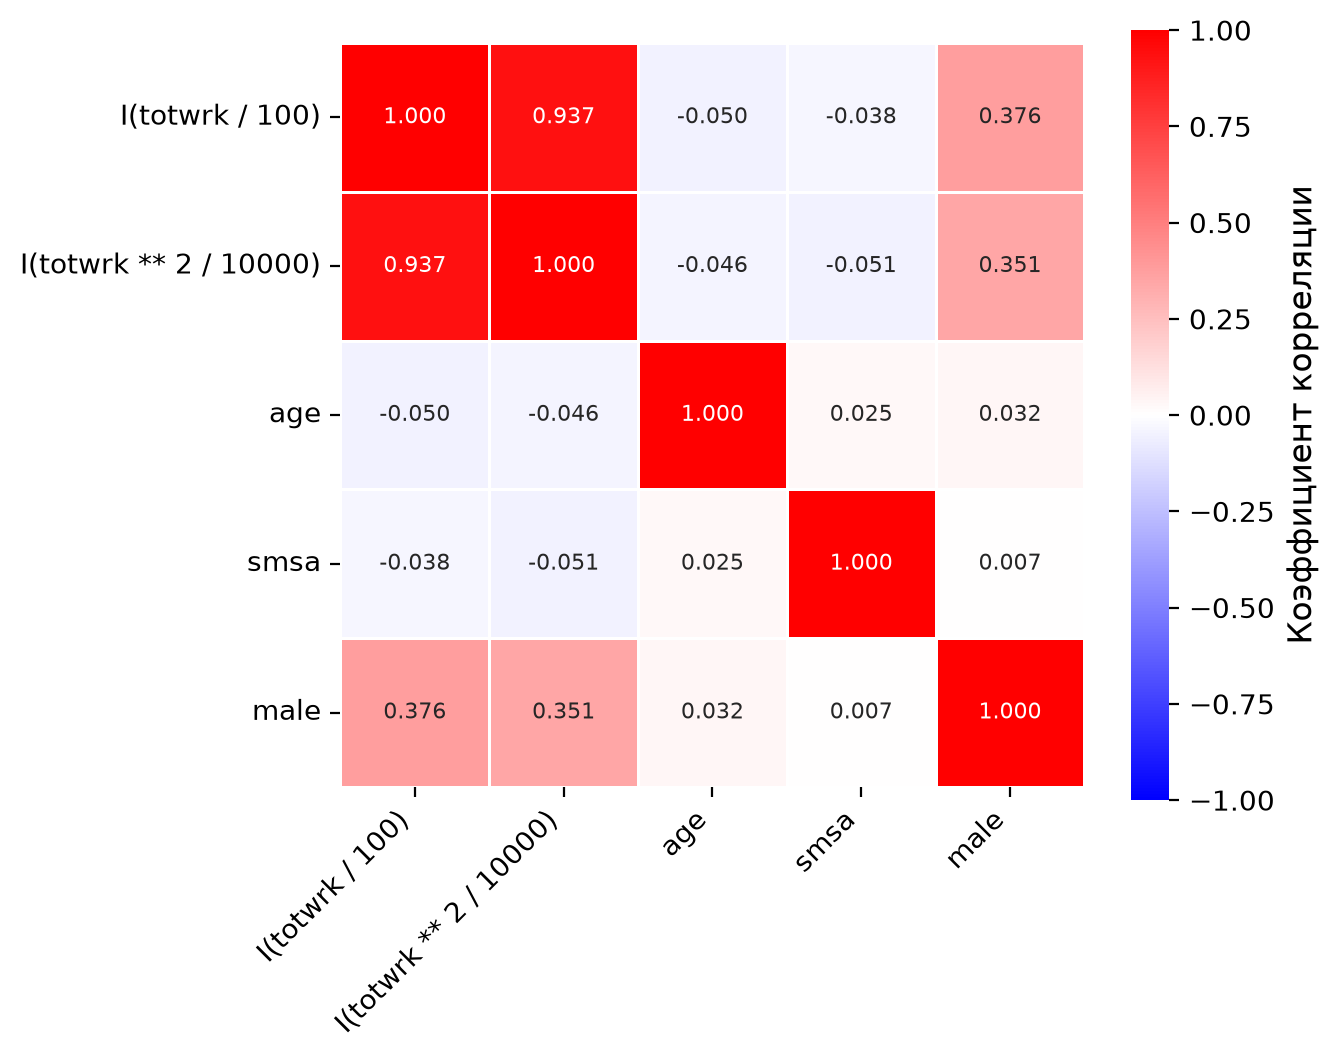
\includegraphics[keepaspectratio]{list09-multicollinearity_files/figure-pdf/fig-corr-sleep1-output-1.png}}

}

\caption{\label{fig-corr-sleep1}Корреляционная матрица регрессоров
(sleep equation \#1)}

\end{figure}%

\begin{tcolorbox}[enhanced jigsaw, arc=.35mm, bottomrule=.15mm, bottomtitle=1mm, breakable, colback=white, colbacktitle=quarto-callout-important-color!10!white, colframe=quarto-callout-important-color-frame, coltitle=black, left=2mm, leftrule=.75mm, opacityback=0, opacitybacktitle=0.6, rightrule=.15mm, title=\textcolor{quarto-callout-important-color}{\faExclamation}\hspace{0.5em}{Условия теста}, titlerule=0mm, toprule=.15mm, toptitle=1mm]

\begin{itemize}
\tightlist
\item
  уровень значимости: \textbf{5\%}
\item
  стандартные ошибки: \textbf{неробастные}
\item
  гипотеза 1: t-тест, значимость каждого коэффициента: \(H_0:\beta_j=0\)
\item
  гипотеза 2: F-тест, значимость влияния занятости:
  \(H_0:\beta_{totwrk/100}=\beta_{totwrk^2/10000}=0\)
\end{itemize}

\end{tcolorbox}

Какие коэффициенты значимы?

\textbf{Результаты \(t\)-теста для коэффициентов (неробастные
стандартные ошибки):}

{\def\LTcaptype{none} % do not increment counter
\begin{longtable}[]{@{}
  >{\raggedright\arraybackslash}p{(\linewidth - 10\tabcolsep) * \real{0.3038}}
  >{\raggedleft\arraybackslash}p{(\linewidth - 10\tabcolsep) * \real{0.1266}}
  >{\raggedleft\arraybackslash}p{(\linewidth - 10\tabcolsep) * \real{0.1519}}
  >{\raggedleft\arraybackslash}p{(\linewidth - 10\tabcolsep) * \real{0.1392}}
  >{\raggedleft\arraybackslash}p{(\linewidth - 10\tabcolsep) * \real{0.1392}}
  >{\raggedright\arraybackslash}p{(\linewidth - 10\tabcolsep) * \real{0.1392}}@{}}
\toprule\noalign{}
\begin{minipage}[b]{\linewidth}\raggedright
\end{minipage} & \begin{minipage}[b]{\linewidth}\raggedleft
Coef.
\end{minipage} & \begin{minipage}[b]{\linewidth}\raggedleft
Std.Err.
\end{minipage} & \begin{minipage}[b]{\linewidth}\raggedleft
t-value
\end{minipage} & \begin{minipage}[b]{\linewidth}\raggedleft
p-value
\end{minipage} & \begin{minipage}[b]{\linewidth}\raggedright
Signif.
\end{minipage} \\
\midrule\noalign{}
\endhead
\bottomrule\noalign{}
\endlastfoot
Intercept & 3428.805 & 76.655 & 44.730 & \textless0.001 & \\
I(totwrk / 100) & -8.195 & 4.789 & -1.711 & 0.088 & * \\
I(totwrk ** 2 / 10000) & -0.214 & 0.111 & -1.930 & 0.054 & * \\
age & 2.817 & 1.387 & 2.031 & 0.043 & ** \\
smsa & -78.049 & 32.072 & -2.434 & 0.015 & ** \\
male & 86.639 & 34.200 & 2.533 & 0.012 & ** \\
\end{longtable}
}

\emph{Signif. codes:} \texttt{***} \(p<0.01\), \texttt{**} \(p<0.05\),
\texttt{*} \(p<0.1\)

\begin{tcolorbox}[enhanced jigsaw, arc=.35mm, bottomrule=.15mm, bottomtitle=1mm, breakable, colback=white, colbacktitle=quarto-callout-note-color!10!white, colframe=quarto-callout-note-color-frame, coltitle=black, left=2mm, leftrule=.75mm, opacityback=0, opacitybacktitle=0.6, rightrule=.15mm, title=\textcolor{quarto-callout-note-color}{\faInfo}\hspace{0.5em}{Коэффициенты, значимые на уровне 5\% (по неробастным стандартным
ошибкам)}, titlerule=0mm, toprule=.15mm, toptitle=1mm]

\texttt{age}, \texttt{smsa}, \texttt{male}

\end{tcolorbox}

Проверим гипотезу о значимости влияния занятости.

\textbf{Результаты \(F\)-теста (неробастные стандартные ошибки):}

{\def\LTcaptype{none} % do not increment counter
\begin{longtable}[]{@{}rrrr@{}}
\toprule\noalign{}
F & df1 & df2 & p-value \\
\midrule\noalign{}
\endhead
\bottomrule\noalign{}
\endlastfoot
45.619 & 2 & 700 & \textless0.001 \\
\end{longtable}
}

Вычислите критическое значение. \textbf{Ответ округлите до 2-х
десятичных знаков.}

\begin{tcolorbox}[enhanced jigsaw, arc=.35mm, bottomrule=.15mm, bottomtitle=1mm, breakable, colback=white, colbacktitle=quarto-callout-note-color!10!white, colframe=quarto-callout-note-color-frame, coltitle=black, left=2mm, leftrule=.75mm, opacityback=0, opacitybacktitle=0.6, rightrule=.15mm, title=\textcolor{quarto-callout-note-color}{\faInfo}\hspace{0.5em}{Критическое значение}, titlerule=0mm, toprule=.15mm, toptitle=1mm]

\(F_{crit} = 3.01\)

\end{tcolorbox}

Какой можно сделать вывод?

\begin{tcolorbox}[enhanced jigsaw, arc=.35mm, bottomrule=.15mm, bottomtitle=1mm, breakable, colback=white, colbacktitle=quarto-callout-tip-color!10!white, colframe=quarto-callout-tip-color-frame, coltitle=black, left=2mm, leftrule=.75mm, opacityback=0, opacitybacktitle=0.6, rightrule=.15mm, title=\textcolor{quarto-callout-tip-color}{\faLightbulb}\hspace{0.5em}{Вывод}, titlerule=0mm, toprule=.15mm, toptitle=1mm]

\(F = 45.619 > 3.01\), гипотеза \(H_0\) отвергается.

\textbf{На первый взгляд противоречие:} коэффициенты при
\texttt{I(totwrk\ /\ 100)} и \texttt{I(totwrk\ **\ 2\ /\ 10000)} по
отдельности незначимы (P-значения 0.088 и 0.054), а гипотеза об их
совместной незначимости отвергается. Оно объясняется
мультиколлинеарностью: корреляция двух регрессоров равна 0.937, VIF ---
8.37 и 8.20.

\end{tcolorbox}

\subsection{sleep equation \#2}\label{sleep-equation-2}

Для набора данных \texttt{sleep75} рассмотрим регрессию

\texttt{sleep\ \textasciitilde{}\ totwrk\ +\ age\ +\ I(age**2)\ +\ smsa\ +\ male\ +\ union}

Модель была подогнана по 706 наблюдениям.

Вычислите показатели VIF для регрессоров. \textbf{Ответ округлите до 2-х
десятичных знаков.}

{\def\LTcaptype{none} % do not increment counter
\begin{longtable}[]{@{}lr@{}}
\toprule\noalign{}
Переменная & VIF \\
\midrule\noalign{}
\endhead
\bottomrule\noalign{}
\endlastfoot
totwrk & 1.20 \\
age & 65.40 \\
I(age ** 2) & 65.56 \\
smsa & 1.00 \\
male & 1.17 \\
union & 1.01 \\
\end{longtable}
}

Вычислите корреляционную матрицу регрессоров. \textbf{Ответ округлите до
3-х десятичных знаков.}

{\def\LTcaptype{none} % do not increment counter
\begin{longtable}[]{@{}
  >{\raggedright\arraybackslash}p{(\linewidth - 12\tabcolsep) * \real{0.1831}}
  >{\raggedleft\arraybackslash}p{(\linewidth - 12\tabcolsep) * \real{0.1408}}
  >{\raggedleft\arraybackslash}p{(\linewidth - 12\tabcolsep) * \real{0.1127}}
  >{\raggedleft\arraybackslash}p{(\linewidth - 12\tabcolsep) * \real{0.2113}}
  >{\raggedleft\arraybackslash}p{(\linewidth - 12\tabcolsep) * \real{0.1127}}
  >{\raggedleft\arraybackslash}p{(\linewidth - 12\tabcolsep) * \real{0.1127}}
  >{\raggedleft\arraybackslash}p{(\linewidth - 12\tabcolsep) * \real{0.1268}}@{}}
\toprule\noalign{}
\begin{minipage}[b]{\linewidth}\raggedright
\end{minipage} & \begin{minipage}[b]{\linewidth}\raggedleft
totwrk
\end{minipage} & \begin{minipage}[b]{\linewidth}\raggedleft
age
\end{minipage} & \begin{minipage}[b]{\linewidth}\raggedleft
I(age ** 2)
\end{minipage} & \begin{minipage}[b]{\linewidth}\raggedleft
smsa
\end{minipage} & \begin{minipage}[b]{\linewidth}\raggedleft
male
\end{minipage} & \begin{minipage}[b]{\linewidth}\raggedleft
union
\end{minipage} \\
\midrule\noalign{}
\endhead
\bottomrule\noalign{}
\endlastfoot
totwrk & 1.000 & -0.050 & -0.067 & -0.038 & 0.376 & 0.002 \\
age & -0.050 & 1.000 & 0.992 & 0.025 & 0.032 & -0.037 \\
I(age ** 2) & -0.067 & 0.992 & 1.000 & 0.024 & 0.026 & -0.042 \\
smsa & -0.038 & 0.025 & 0.024 & 1.000 & 0.007 & -0.039 \\
male & 0.376 & 0.032 & 0.026 & 0.007 & 1.000 & 0.040 \\
union & 0.002 & -0.037 & -0.042 & -0.039 & 0.040 & 1.000 \\
\end{longtable}
}

Постройте тепловую карту корреляционной матрицы
(Рисунок~\ref{fig-corr-sleep2}).

\begin{figure}

\centering{

\pandocbounded{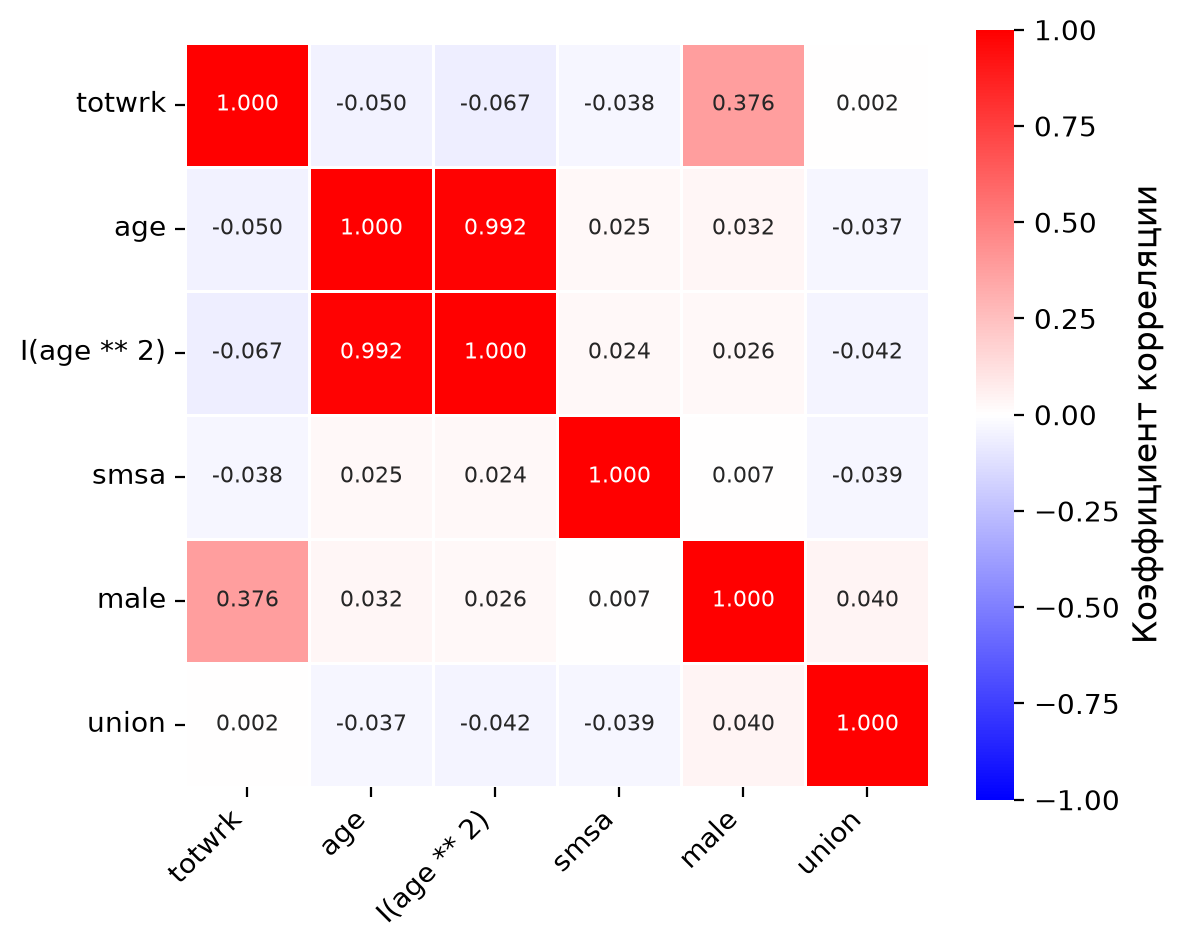
\includegraphics[keepaspectratio]{list09-multicollinearity_files/figure-pdf/fig-corr-sleep2-output-1.png}}

}

\caption{\label{fig-corr-sleep2}Корреляционная матрица регрессоров
(sleep equation \#2)}

\end{figure}%

\begin{tcolorbox}[enhanced jigsaw, arc=.35mm, bottomrule=.15mm, bottomtitle=1mm, breakable, colback=white, colbacktitle=quarto-callout-important-color!10!white, colframe=quarto-callout-important-color-frame, coltitle=black, left=2mm, leftrule=.75mm, opacityback=0, opacitybacktitle=0.6, rightrule=.15mm, title=\textcolor{quarto-callout-important-color}{\faExclamation}\hspace{0.5em}{Условия теста}, titlerule=0mm, toprule=.15mm, toptitle=1mm]

\begin{itemize}
\tightlist
\item
  уровень значимости: \textbf{5\% и 10\%}
\item
  стандартные ошибки: \textbf{неробастные}
\item
  гипотеза 1: t-тест, значимость каждого коэффициента: \(H_0:\beta_j=0\)
\item
  гипотеза 2: F-тест, значимость влияния возраста:
  \(H_0:\beta_{age}=\beta_{age^2}=0\)
\end{itemize}

\end{tcolorbox}

Какие коэффициенты значимы на каждом из двух уровней?

\textbf{Результаты \(t\)-теста для коэффициентов (неробастные
стандартные ошибки):}

{\def\LTcaptype{none} % do not increment counter
\begin{longtable}[]{@{}
  >{\raggedright\arraybackslash}p{(\linewidth - 10\tabcolsep) * \real{0.1912}}
  >{\raggedleft\arraybackslash}p{(\linewidth - 10\tabcolsep) * \real{0.1471}}
  >{\raggedleft\arraybackslash}p{(\linewidth - 10\tabcolsep) * \real{0.1765}}
  >{\raggedleft\arraybackslash}p{(\linewidth - 10\tabcolsep) * \real{0.1618}}
  >{\raggedleft\arraybackslash}p{(\linewidth - 10\tabcolsep) * \real{0.1618}}
  >{\raggedright\arraybackslash}p{(\linewidth - 10\tabcolsep) * \real{0.1618}}@{}}
\toprule\noalign{}
\begin{minipage}[b]{\linewidth}\raggedright
\end{minipage} & \begin{minipage}[b]{\linewidth}\raggedleft
Coef.
\end{minipage} & \begin{minipage}[b]{\linewidth}\raggedleft
Std.Err.
\end{minipage} & \begin{minipage}[b]{\linewidth}\raggedleft
t-value
\end{minipage} & \begin{minipage}[b]{\linewidth}\raggedleft
p-value
\end{minipage} & \begin{minipage}[b]{\linewidth}\raggedright
Signif.
\end{minipage} \\
\midrule\noalign{}
\endhead
\bottomrule\noalign{}
\endlastfoot
Intercept & 3688.551 & 218.389 & 16.890 & \textless0.001 & \\
totwrk & -0.165 & 0.018 & -9.105 & \textless0.001 & *** \\
age & -7.734 & 11.213 & -0.690 & 0.491 & \\
I(age ** 2) & 0.127 & 0.134 & 0.948 & 0.343 & \\
smsa & -74.527 & 32.156 & -2.318 & 0.021 & ** \\
male & 86.321 & 34.329 & 2.515 & 0.012 & ** \\
union & 8.574 & 38.195 & 0.224 & 0.822 & \\
\end{longtable}
}

\emph{Signif. codes:} \texttt{***} \(p<0.01\), \texttt{**} \(p<0.05\),
\texttt{*} \(p<0.1\)

\begin{tcolorbox}[enhanced jigsaw, arc=.35mm, bottomrule=.15mm, bottomtitle=1mm, breakable, colback=white, colbacktitle=quarto-callout-note-color!10!white, colframe=quarto-callout-note-color-frame, coltitle=black, left=2mm, leftrule=.75mm, opacityback=0, opacitybacktitle=0.6, rightrule=.15mm, title=\textcolor{quarto-callout-note-color}{\faInfo}\hspace{0.5em}{Значимые коэффициенты (по неробастным стандартным ошибкам)}, titlerule=0mm, toprule=.15mm, toptitle=1mm]

\begin{itemize}
\tightlist
\item
  на уровне 5\%: \texttt{totwrk}, \texttt{smsa}, \texttt{male}
\item
  на уровне 10\%: \texttt{totwrk}, \texttt{smsa}, \texttt{male}
\end{itemize}

\end{tcolorbox}

Проверим гипотезу о значимости влияния возраста.

\textbf{Результаты \(F\)-теста (неробастные стандартные ошибки):}

{\def\LTcaptype{none} % do not increment counter
\begin{longtable}[]{@{}rrrr@{}}
\toprule\noalign{}
F & df1 & df2 & p-value \\
\midrule\noalign{}
\endhead
\bottomrule\noalign{}
\endlastfoot
2.497 & 2 & 699 & 0.083 \\
\end{longtable}
}

Вычислите критические значения для двух уровней значимости.
\textbf{Ответ округлите до 2-х десятичных знаков.}

\begin{tcolorbox}[enhanced jigsaw, arc=.35mm, bottomrule=.15mm, bottomtitle=1mm, breakable, colback=white, colbacktitle=quarto-callout-note-color!10!white, colframe=quarto-callout-note-color-frame, coltitle=black, left=2mm, leftrule=.75mm, opacityback=0, opacitybacktitle=0.6, rightrule=.15mm, title=\textcolor{quarto-callout-note-color}{\faInfo}\hspace{0.5em}{Критические значения}, titlerule=0mm, toprule=.15mm, toptitle=1mm]

\begin{itemize}
\tightlist
\item
  уровень значимости 5\%: \(F_{crit} = 3.01\)
\item
  уровень значимости 10\%: \(F_{crit} = 2.31\)
\end{itemize}

\end{tcolorbox}

Какой можно сделать вывод на каждом из двух уровней?

\begin{tcolorbox}[enhanced jigsaw, arc=.35mm, bottomrule=.15mm, bottomtitle=1mm, breakable, colback=white, colbacktitle=quarto-callout-tip-color!10!white, colframe=quarto-callout-tip-color-frame, coltitle=black, left=2mm, leftrule=.75mm, opacityback=0, opacitybacktitle=0.6, rightrule=.15mm, title=\textcolor{quarto-callout-tip-color}{\faLightbulb}\hspace{0.5em}{Вывод}, titlerule=0mm, toprule=.15mm, toptitle=1mm]

\begin{itemize}
\tightlist
\item
  На уровне 5\%: \(F = 2.497 < 3.01\), гипотеза \(H_0\) не отвергается.
  Противоречия нет: коэффициенты при \texttt{age} и
  \texttt{I(age\ **\ 2)} незначимы по отдельности (P-значения 0.491 и
  0.343), и гипотеза об их совместной незначимости тоже не отвергается.
\item
  На уровне 10\%: \(F = 2.497 > 2.31\), гипотеза \(H_0\) отвергается,
  хотя коэффициенты при \texttt{age} и \texttt{I(age\ **\ 2)} по
  отдельности незначимы. \textbf{На первый взгляд противоречие.} Оно
  объясняется мультиколлинеарностью: корреляция \texttt{age} и
  \texttt{I(age\ **\ 2)} равна 0.992, VIF --- 65.40 и 65.56.
\end{itemize}

\end{tcolorbox}

\subsection{sleep equation \#3}\label{sleep-equation-3}

Для набора данных \texttt{sleep75} рассмотрим регрессию

\begin{verbatim}
sleep ~ totwrk + age + smsa + south +
        I(totwrk*south) + I(age*south) + I(smsa*south)
\end{verbatim}

Модель была подогнана по 706 наблюдениям.

Вычислите показатели VIF для регрессоров. \textbf{Ответ округлите до 2-х
десятичных знаков.}

{\def\LTcaptype{none} % do not increment counter
\begin{longtable}[]{@{}lr@{}}
\toprule\noalign{}
Переменная & VIF \\
\midrule\noalign{}
\endhead
\bottomrule\noalign{}
\endlastfoot
totwrk & 1.15 \\
age & 1.25 \\
smsa & 1.19 \\
south & 22.00 \\
I(totwrk * south) & 8.85 \\
I(age * south) & 12.28 \\
I(smsa * south) & 1.29 \\
\end{longtable}
}

Вычислите корреляционную матрицу регрессоров. \textbf{Ответ округлите до
3-х десятичных знаков.}

{\def\LTcaptype{none} % do not increment counter
\begin{longtable}[]{@{}
  >{\raggedright\arraybackslash}p{(\linewidth - 14\tabcolsep) * \real{0.1696}}
  >{\raggedleft\arraybackslash}p{(\linewidth - 14\tabcolsep) * \real{0.0893}}
  >{\raggedleft\arraybackslash}p{(\linewidth - 14\tabcolsep) * \real{0.0714}}
  >{\raggedleft\arraybackslash}p{(\linewidth - 14\tabcolsep) * \real{0.0714}}
  >{\raggedleft\arraybackslash}p{(\linewidth - 14\tabcolsep) * \real{0.0804}}
  >{\raggedleft\arraybackslash}p{(\linewidth - 14\tabcolsep) * \real{0.1875}}
  >{\raggedleft\arraybackslash}p{(\linewidth - 14\tabcolsep) * \real{0.1607}}
  >{\raggedleft\arraybackslash}p{(\linewidth - 14\tabcolsep) * \real{0.1696}}@{}}
\toprule\noalign{}
\begin{minipage}[b]{\linewidth}\raggedright
\end{minipage} & \begin{minipage}[b]{\linewidth}\raggedleft
totwrk
\end{minipage} & \begin{minipage}[b]{\linewidth}\raggedleft
age
\end{minipage} & \begin{minipage}[b]{\linewidth}\raggedleft
smsa
\end{minipage} & \begin{minipage}[b]{\linewidth}\raggedleft
south
\end{minipage} & \begin{minipage}[b]{\linewidth}\raggedleft
I(totwrk * south)
\end{minipage} & \begin{minipage}[b]{\linewidth}\raggedleft
I(age * south)
\end{minipage} & \begin{minipage}[b]{\linewidth}\raggedleft
I(smsa * south)
\end{minipage} \\
\midrule\noalign{}
\endhead
\bottomrule\noalign{}
\endlastfoot
totwrk & 1.000 & -0.050 & -0.038 & 0.051 & 0.175 & 0.033 & 0.012 \\
age & -0.050 & 1.000 & 0.025 & -0.018 & -0.038 & 0.126 & 0.008 \\
smsa & -0.038 & 0.025 & 1.000 & -0.238 & -0.224 & -0.222 & 0.209 \\
south & 0.051 & -0.018 & -0.238 & 1.000 & 0.932 & 0.947 & 0.359 \\
I(totwrk * south) & 0.175 & -0.038 & -0.224 & 0.932 & 1.000 & 0.868 &
0.328 \\
I(age * south) & 0.033 & 0.126 & -0.222 & 0.947 & 0.868 & 1.000 &
0.351 \\
I(smsa * south) & 0.012 & 0.008 & 0.209 & 0.359 & 0.328 & 0.351 &
1.000 \\
\end{longtable}
}

Постройте тепловую карту корреляционной матрицы
(Рисунок~\ref{fig-corr-sleep3}).

\begin{figure}

\centering{

\pandocbounded{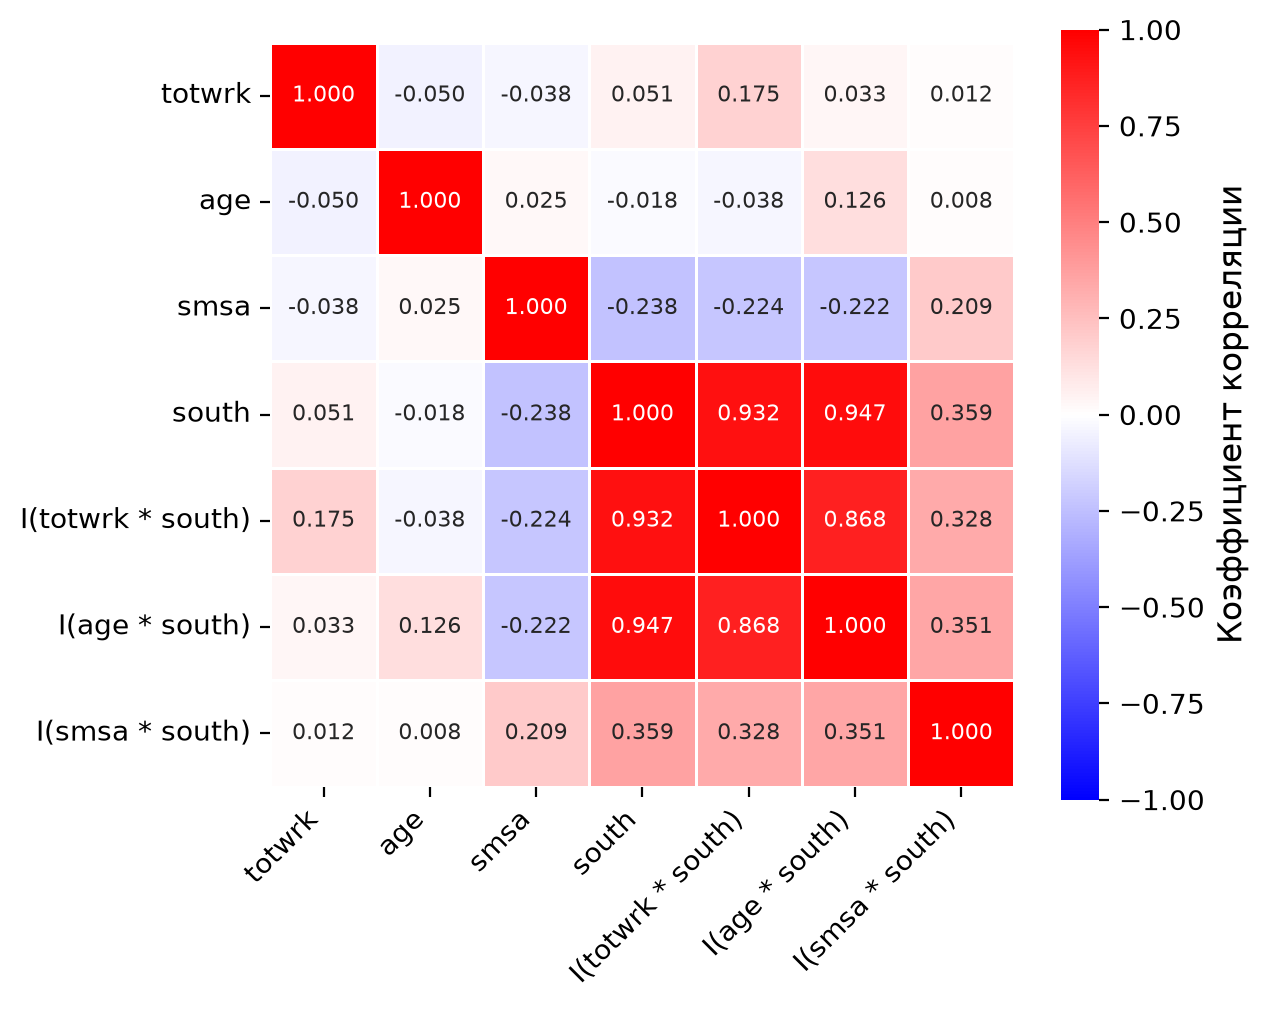
\includegraphics[keepaspectratio]{list09-multicollinearity_files/figure-pdf/fig-corr-sleep3-output-1.png}}

}

\caption{\label{fig-corr-sleep3}Корреляционная матрица регрессоров
(sleep equation \#3)}

\end{figure}%

\begin{tcolorbox}[enhanced jigsaw, arc=.35mm, bottomrule=.15mm, bottomtitle=1mm, breakable, colback=white, colbacktitle=quarto-callout-important-color!10!white, colframe=quarto-callout-important-color-frame, coltitle=black, left=2mm, leftrule=.75mm, opacityback=0, opacitybacktitle=0.6, rightrule=.15mm, title=\textcolor{quarto-callout-important-color}{\faExclamation}\hspace{0.5em}{Условия теста}, titlerule=0mm, toprule=.15mm, toptitle=1mm]

\begin{itemize}
\tightlist
\item
  уровень значимости: \textbf{5\%}
\item
  стандартные ошибки: \textbf{неробастные}
\item
  гипотеза 1: t-тест, значимость каждого коэффициента: \(H_0:\beta_j=0\)
\item
  гипотеза 2: F-тест, значимость региона (переменная \texttt{south}):
  \(H_0:\beta_{south}=\beta_{totwrk\cdot south}=\beta_{age\cdot south}=\beta_{smsa\cdot south}=0\)
\end{itemize}

\end{tcolorbox}

Какие коэффициенты значимы?

\textbf{Результаты \(t\)-теста для коэффициентов (неробастные
стандартные ошибки):}

{\def\LTcaptype{none} % do not increment counter
\begin{longtable}[]{@{}
  >{\raggedright\arraybackslash}p{(\linewidth - 10\tabcolsep) * \real{0.2568}}
  >{\raggedleft\arraybackslash}p{(\linewidth - 10\tabcolsep) * \real{0.1351}}
  >{\raggedleft\arraybackslash}p{(\linewidth - 10\tabcolsep) * \real{0.1622}}
  >{\raggedleft\arraybackslash}p{(\linewidth - 10\tabcolsep) * \real{0.1486}}
  >{\raggedleft\arraybackslash}p{(\linewidth - 10\tabcolsep) * \real{0.1486}}
  >{\raggedright\arraybackslash}p{(\linewidth - 10\tabcolsep) * \real{0.1486}}@{}}
\toprule\noalign{}
\begin{minipage}[b]{\linewidth}\raggedright
\end{minipage} & \begin{minipage}[b]{\linewidth}\raggedleft
Coef.
\end{minipage} & \begin{minipage}[b]{\linewidth}\raggedleft
Std.Err.
\end{minipage} & \begin{minipage}[b]{\linewidth}\raggedleft
t-value
\end{minipage} & \begin{minipage}[b]{\linewidth}\raggedleft
p-value
\end{minipage} & \begin{minipage}[b]{\linewidth}\raggedright
Signif.
\end{minipage} \\
\midrule\noalign{}
\endhead
\bottomrule\noalign{}
\endlastfoot
Intercept & 3557.513 & 75.504 & 47.117 & \textless0.001 & \\
totwrk & -0.161 & 0.018 & -9.062 & \textless0.001 & *** \\
age & 1.485 & 1.545 & 0.961 & 0.337 & \\
smsa & -61.554 & 34.856 & -1.766 & 0.078 & * \\
south & -407.206 & 189.627 & -2.147 & 0.032 & ** \\
I(totwrk * south) & 0.078 & 0.050 & 1.556 & 0.120 & \\
I(age * south) & 8.267 & 3.495 & 2.365 & 0.018 & ** \\
I(smsa * south) & 49.429 & 107.111 & 0.461 & 0.645 & \\
\end{longtable}
}

\emph{Signif. codes:} \texttt{***} \(p<0.01\), \texttt{**} \(p<0.05\),
\texttt{*} \(p<0.1\)

\begin{tcolorbox}[enhanced jigsaw, arc=.35mm, bottomrule=.15mm, bottomtitle=1mm, breakable, colback=white, colbacktitle=quarto-callout-note-color!10!white, colframe=quarto-callout-note-color-frame, coltitle=black, left=2mm, leftrule=.75mm, opacityback=0, opacitybacktitle=0.6, rightrule=.15mm, title=\textcolor{quarto-callout-note-color}{\faInfo}\hspace{0.5em}{Коэффициенты, значимые на уровне 5\% (по неробастным стандартным
ошибкам)}, titlerule=0mm, toprule=.15mm, toptitle=1mm]

\texttt{totwrk}, \texttt{south}, \texttt{I(age\ *\ south)}

\end{tcolorbox}

Проверим гипотезу о значимости региона.

\textbf{Результаты \(F\)-теста (неробастные стандартные ошибки):}

{\def\LTcaptype{none} % do not increment counter
\begin{longtable}[]{@{}rrrr@{}}
\toprule\noalign{}
F & df1 & df2 & p-value \\
\midrule\noalign{}
\endhead
\bottomrule\noalign{}
\endlastfoot
3.144 & 4 & 698 & 0.014 \\
\end{longtable}
}

Вычислите критическое значение. \textbf{Ответ округлите до 2-х
десятичных знаков.}

\begin{tcolorbox}[enhanced jigsaw, arc=.35mm, bottomrule=.15mm, bottomtitle=1mm, breakable, colback=white, colbacktitle=quarto-callout-note-color!10!white, colframe=quarto-callout-note-color-frame, coltitle=black, left=2mm, leftrule=.75mm, opacityback=0, opacitybacktitle=0.6, rightrule=.15mm, title=\textcolor{quarto-callout-note-color}{\faInfo}\hspace{0.5em}{Критическое значение}, titlerule=0mm, toprule=.15mm, toptitle=1mm]

\(F_{crit} = 2.38\)

\end{tcolorbox}

Какой можно сделать вывод?

\begin{tcolorbox}[enhanced jigsaw, arc=.35mm, bottomrule=.15mm, bottomtitle=1mm, breakable, colback=white, colbacktitle=quarto-callout-tip-color!10!white, colframe=quarto-callout-tip-color-frame, coltitle=black, left=2mm, leftrule=.75mm, opacityback=0, opacitybacktitle=0.6, rightrule=.15mm, title=\textcolor{quarto-callout-tip-color}{\faLightbulb}\hspace{0.5em}{Вывод}, titlerule=0mm, toprule=.15mm, toptitle=1mm]

\(F = 3.144 > 2.38\), гипотеза \(H_0\) отвергается.

Здесь противоречия нет: коэффициенты при \texttt{south} и
\texttt{I(age\ *\ south)} значимы и по отдельности (P-значения 0.032 и
0.018), а F-тест отвергает совместную незначимость всех четырёх. При
этом VIF у \texttt{south} равен 22.00, у \texttt{I(age\ *\ south)} ---
12.28: высокий VIF увеличивает стандартные ошибки, но сам по себе не
делает коэффициент незначимым.

\end{tcolorbox}

\subsection{wage equation \#1}\label{wage-equation-1}

Для набора данных \texttt{wage2} рассмотрим регрессию

\texttt{np.log(wage)\ \textasciitilde{}\ age\ +\ I(age**2)\ +\ IQ\ +\ married\ +\ south\ +\ urban}

Переменная \texttt{wage} --- месячный заработок, \texttt{age} ---
возраст в годах, \texttt{IQ} --- результат теста IQ; \texttt{married},
\texttt{south}, \texttt{urban} --- бинарные переменные.

Модель была подогнана по 935 наблюдениям.

Вычислите показатели VIF для регрессоров. \textbf{Ответ округлите до 2-х
десятичных знаков.}

{\def\LTcaptype{none} % do not increment counter
\begin{longtable}[]{@{}lr@{}}
\toprule\noalign{}
Переменная & VIF \\
\midrule\noalign{}
\endhead
\bottomrule\noalign{}
\endlastfoot
age & 632.87 \\
I(age ** 2) & 632.96 \\
IQ & 1.05 \\
married & 1.01 \\
south & 1.06 \\
urban & 1.02 \\
\end{longtable}
}

Вычислите корреляционную матрицу регрессоров. \textbf{Ответ округлите до
3-х десятичных знаков.}

{\def\LTcaptype{none} % do not increment counter
\begin{longtable}[]{@{}
  >{\raggedright\arraybackslash}p{(\linewidth - 12\tabcolsep) * \real{0.1781}}
  >{\raggedleft\arraybackslash}p{(\linewidth - 12\tabcolsep) * \real{0.1096}}
  >{\raggedleft\arraybackslash}p{(\linewidth - 12\tabcolsep) * \real{0.2055}}
  >{\raggedleft\arraybackslash}p{(\linewidth - 12\tabcolsep) * \real{0.1096}}
  >{\raggedleft\arraybackslash}p{(\linewidth - 12\tabcolsep) * \real{0.1507}}
  >{\raggedleft\arraybackslash}p{(\linewidth - 12\tabcolsep) * \real{0.1233}}
  >{\raggedleft\arraybackslash}p{(\linewidth - 12\tabcolsep) * \real{0.1233}}@{}}
\toprule\noalign{}
\begin{minipage}[b]{\linewidth}\raggedright
\end{minipage} & \begin{minipage}[b]{\linewidth}\raggedleft
age
\end{minipage} & \begin{minipage}[b]{\linewidth}\raggedleft
I(age ** 2)
\end{minipage} & \begin{minipage}[b]{\linewidth}\raggedleft
IQ
\end{minipage} & \begin{minipage}[b]{\linewidth}\raggedleft
married
\end{minipage} & \begin{minipage}[b]{\linewidth}\raggedleft
south
\end{minipage} & \begin{minipage}[b]{\linewidth}\raggedleft
urban
\end{minipage} \\
\midrule\noalign{}
\endhead
\bottomrule\noalign{}
\endlastfoot
age & 1.000 & 0.999 & -0.044 & 0.107 & -0.029 & -0.007 \\
I(age ** 2) & 0.999 & 1.000 & -0.043 & 0.107 & -0.031 & -0.009 \\
IQ & -0.044 & -0.043 & 1.000 & -0.015 & -0.210 & 0.039 \\
married & 0.107 & 0.107 & -0.015 & 1.000 & 0.023 & -0.040 \\
south & -0.029 & -0.031 & -0.210 & 0.023 & 1.000 & -0.110 \\
urban & -0.007 & -0.009 & 0.039 & -0.040 & -0.110 & 1.000 \\
\end{longtable}
}

Постройте тепловую карту корреляционной матрицы
(Рисунок~\ref{fig-corr-wage1}).

\begin{figure}

\centering{

\pandocbounded{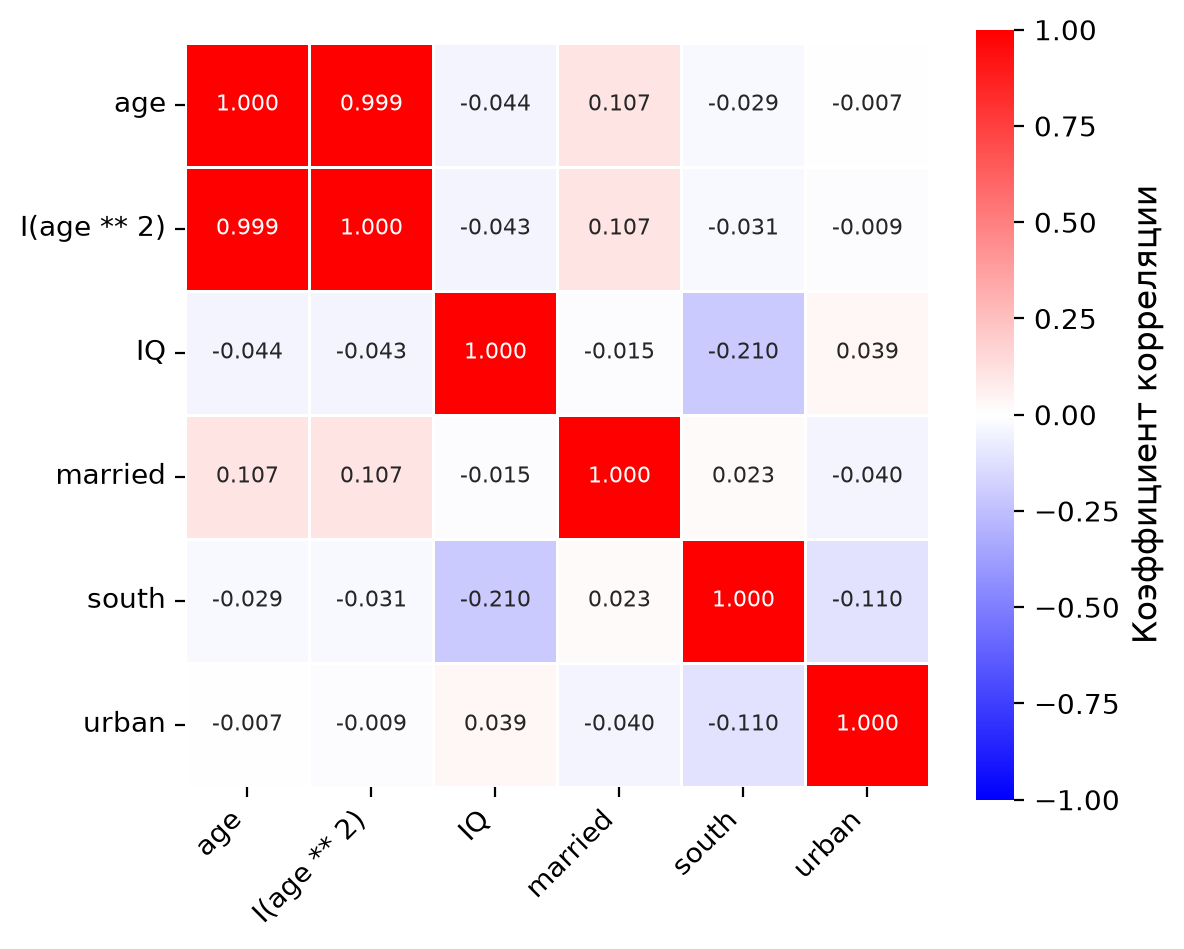
\includegraphics[keepaspectratio]{list09-multicollinearity_files/figure-pdf/fig-corr-wage1-output-1.png}}

}

\caption{\label{fig-corr-wage1}Корреляционная матрица регрессоров (wage
equation \#1)}

\end{figure}%

\begin{tcolorbox}[enhanced jigsaw, arc=.35mm, bottomrule=.15mm, bottomtitle=1mm, breakable, colback=white, colbacktitle=quarto-callout-important-color!10!white, colframe=quarto-callout-important-color-frame, coltitle=black, left=2mm, leftrule=.75mm, opacityback=0, opacitybacktitle=0.6, rightrule=.15mm, title=\textcolor{quarto-callout-important-color}{\faExclamation}\hspace{0.5em}{Условия теста}, titlerule=0mm, toprule=.15mm, toptitle=1mm]

\begin{itemize}
\tightlist
\item
  уровень значимости: \textbf{5\%}
\item
  стандартные ошибки: \textbf{неробастные}
\item
  гипотеза 1: t-тест, значимость каждого коэффициента: \(H_0:\beta_j=0\)
\item
  гипотеза 2: F-тест, значимость влияния возраста:
  \(H_0:\beta_{age}=\beta_{age^2}=0\)
\end{itemize}

\end{tcolorbox}

Какие коэффициенты значимы?

\textbf{Результаты \(t\)-теста для коэффициентов (неробастные
стандартные ошибки):}

{\def\LTcaptype{none} % do not increment counter
\begin{longtable}[]{@{}
  >{\raggedright\arraybackslash}p{(\linewidth - 10\tabcolsep) * \real{0.1940}}
  >{\raggedleft\arraybackslash}p{(\linewidth - 10\tabcolsep) * \real{0.1343}}
  >{\raggedleft\arraybackslash}p{(\linewidth - 10\tabcolsep) * \real{0.1791}}
  >{\raggedleft\arraybackslash}p{(\linewidth - 10\tabcolsep) * \real{0.1642}}
  >{\raggedleft\arraybackslash}p{(\linewidth - 10\tabcolsep) * \real{0.1642}}
  >{\raggedright\arraybackslash}p{(\linewidth - 10\tabcolsep) * \real{0.1642}}@{}}
\toprule\noalign{}
\begin{minipage}[b]{\linewidth}\raggedright
\end{minipage} & \begin{minipage}[b]{\linewidth}\raggedleft
Coef.
\end{minipage} & \begin{minipage}[b]{\linewidth}\raggedleft
Std.Err.
\end{minipage} & \begin{minipage}[b]{\linewidth}\raggedleft
t-value
\end{minipage} & \begin{minipage}[b]{\linewidth}\raggedleft
p-value
\end{minipage} & \begin{minipage}[b]{\linewidth}\raggedright
Signif.
\end{minipage} \\
\midrule\noalign{}
\endhead
\bottomrule\noalign{}
\endlastfoot
Intercept & 2.938 & 1.656 & 1.774 & 0.076 & \\
age & 0.145 & 0.100 & 1.447 & 0.148 & \\
I(age ** 2) & -0.002 & 0.002 & -1.236 & 0.217 & \\
IQ & 0.008 & 0.001 & 9.770 & \textless0.001 & *** \\
married & 0.202 & 0.040 & 5.008 & \textless0.001 & *** \\
south & -0.100 & 0.027 & -3.736 & \textless0.001 & *** \\
urban & 0.173 & 0.028 & 6.260 & \textless0.001 & *** \\
\end{longtable}
}

\emph{Signif. codes:} \texttt{***} \(p<0.01\), \texttt{**} \(p<0.05\),
\texttt{*} \(p<0.1\)

\begin{tcolorbox}[enhanced jigsaw, arc=.35mm, bottomrule=.15mm, bottomtitle=1mm, breakable, colback=white, colbacktitle=quarto-callout-note-color!10!white, colframe=quarto-callout-note-color-frame, coltitle=black, left=2mm, leftrule=.75mm, opacityback=0, opacitybacktitle=0.6, rightrule=.15mm, title=\textcolor{quarto-callout-note-color}{\faInfo}\hspace{0.5em}{Коэффициенты, значимые на уровне 5\% (по неробастным стандартным
ошибкам)}, titlerule=0mm, toprule=.15mm, toptitle=1mm]

\texttt{IQ}, \texttt{married}, \texttt{south}, \texttt{urban}

\end{tcolorbox}

Проверим гипотезу о значимости влияния возраста.

\textbf{Результаты \(F\)-теста (неробастные стандартные ошибки):}

{\def\LTcaptype{none} % do not increment counter
\begin{longtable}[]{@{}rrrr@{}}
\toprule\noalign{}
F & df1 & df2 & p-value \\
\midrule\noalign{}
\endhead
\bottomrule\noalign{}
\endlastfoot
14.833 & 2 & 928 & \textless0.001 \\
\end{longtable}
}

Вычислите критическое значение. \textbf{Ответ округлите до 2-х
десятичных знаков.}

\begin{tcolorbox}[enhanced jigsaw, arc=.35mm, bottomrule=.15mm, bottomtitle=1mm, breakable, colback=white, colbacktitle=quarto-callout-note-color!10!white, colframe=quarto-callout-note-color-frame, coltitle=black, left=2mm, leftrule=.75mm, opacityback=0, opacitybacktitle=0.6, rightrule=.15mm, title=\textcolor{quarto-callout-note-color}{\faInfo}\hspace{0.5em}{Критическое значение}, titlerule=0mm, toprule=.15mm, toptitle=1mm]

\(F_{crit} = 3.01\)

\end{tcolorbox}

Какой можно сделать вывод?

\begin{tcolorbox}[enhanced jigsaw, arc=.35mm, bottomrule=.15mm, bottomtitle=1mm, breakable, colback=white, colbacktitle=quarto-callout-tip-color!10!white, colframe=quarto-callout-tip-color-frame, coltitle=black, left=2mm, leftrule=.75mm, opacityback=0, opacitybacktitle=0.6, rightrule=.15mm, title=\textcolor{quarto-callout-tip-color}{\faLightbulb}\hspace{0.5em}{Вывод}, titlerule=0mm, toprule=.15mm, toptitle=1mm]

\(F = 14.833 > 3.01\), гипотеза \(H_0\) отвергается.

\textbf{На первый взгляд противоречие:} коэффициенты при \texttt{age} и
\texttt{I(age\ **\ 2)} по отдельности незначимы (P-значения 0.148 и
0.217), а гипотеза об их совместной незначимости отвергается. Оно
объясняется мультиколлинеарностью: корреляция \texttt{age} и
\texttt{I(age\ **\ 2)} равна 0.999, VIF --- 632.87 и 632.96.

\end{tcolorbox}

\subsection{wage equation \#2}\label{wage-equation-2}

Для набора данных \texttt{wage2} рассмотрим регрессию

\begin{verbatim}
np.log(wage) ~ age + IQ + south + urban +
               I(age*urban) + I(IQ*urban) + I(south*urban)
\end{verbatim}

Модель была подогнана по 935 наблюдениям.

Вычислите показатели VIF для регрессоров. \textbf{Ответ округлите до 2-х
десятичных знаков.}

{\def\LTcaptype{none} % do not increment counter
\begin{longtable}[]{@{}lr@{}}
\toprule\noalign{}
Переменная & VIF \\
\midrule\noalign{}
\endhead
\bottomrule\noalign{}
\endlastfoot
age & 3.39 \\
IQ & 3.88 \\
south & 3.83 \\
urban & 175.88 \\
I(age * urban) & 114.32 \\
I(IQ * urban) & 53.14 \\
I(south * urban) & 4.09 \\
\end{longtable}
}

Вычислите корреляционную матрицу регрессоров. \textbf{Ответ округлите до
3-х десятичных знаков.}

{\def\LTcaptype{none} % do not increment counter
\begin{longtable}[]{@{}
  >{\raggedright\arraybackslash}p{(\linewidth - 14\tabcolsep) * \real{0.1682}}
  >{\raggedleft\arraybackslash}p{(\linewidth - 14\tabcolsep) * \real{0.0748}}
  >{\raggedleft\arraybackslash}p{(\linewidth - 14\tabcolsep) * \real{0.0748}}
  >{\raggedleft\arraybackslash}p{(\linewidth - 14\tabcolsep) * \real{0.0841}}
  >{\raggedleft\arraybackslash}p{(\linewidth - 14\tabcolsep) * \real{0.0841}}
  >{\raggedleft\arraybackslash}p{(\linewidth - 14\tabcolsep) * \real{0.1682}}
  >{\raggedleft\arraybackslash}p{(\linewidth - 14\tabcolsep) * \real{0.1589}}
  >{\raggedleft\arraybackslash}p{(\linewidth - 14\tabcolsep) * \real{0.1869}}@{}}
\toprule\noalign{}
\begin{minipage}[b]{\linewidth}\raggedright
\end{minipage} & \begin{minipage}[b]{\linewidth}\raggedleft
age
\end{minipage} & \begin{minipage}[b]{\linewidth}\raggedleft
IQ
\end{minipage} & \begin{minipage}[b]{\linewidth}\raggedleft
south
\end{minipage} & \begin{minipage}[b]{\linewidth}\raggedleft
urban
\end{minipage} & \begin{minipage}[b]{\linewidth}\raggedleft
I(age * urban)
\end{minipage} & \begin{minipage}[b]{\linewidth}\raggedleft
I(IQ * urban)
\end{minipage} & \begin{minipage}[b]{\linewidth}\raggedleft
I(south * urban)
\end{minipage} \\
\midrule\noalign{}
\endhead
\bottomrule\noalign{}
\endlastfoot
age & 1.000 & -0.044 & -0.029 & -0.007 & 0.137 & -0.020 & 0.010 \\
IQ & -0.044 & 1.000 & -0.210 & 0.039 & 0.030 & 0.260 & -0.097 \\
south & -0.029 & -0.210 & 1.000 & -0.110 & -0.106 & -0.136 & 0.741 \\
urban & -0.007 & 0.039 & -0.110 & 1.000 & 0.985 & 0.964 & 0.334 \\
I(age * urban) & 0.137 & 0.030 & -0.106 & 0.985 & 1.000 & 0.947 &
0.332 \\
I(IQ * urban) & -0.020 & 0.260 & -0.136 & 0.964 & 0.947 & 1.000 &
0.288 \\
I(south * urban) & 0.010 & -0.097 & 0.741 & 0.334 & 0.332 & 0.288 &
1.000 \\
\end{longtable}
}

Постройте тепловую карту корреляционной матрицы
(Рисунок~\ref{fig-corr-wage2}).

\begin{figure}

\centering{

\pandocbounded{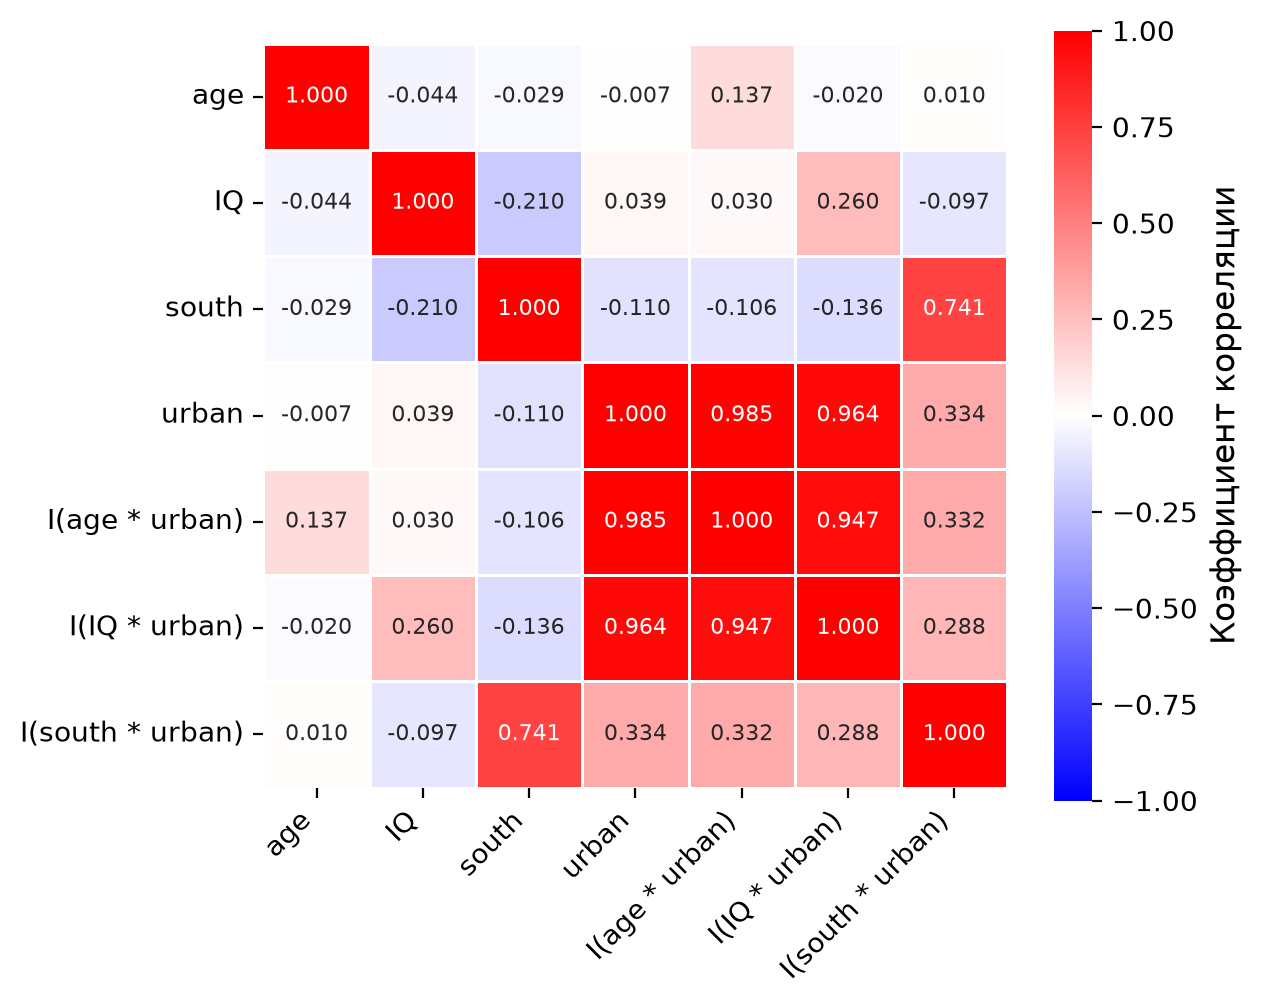
\includegraphics[keepaspectratio]{list09-multicollinearity_files/figure-pdf/fig-corr-wage2-output-1.png}}

}

\caption{\label{fig-corr-wage2}Корреляционная матрица регрессоров (wage
equation \#2)}

\end{figure}%

\begin{tcolorbox}[enhanced jigsaw, arc=.35mm, bottomrule=.15mm, bottomtitle=1mm, breakable, colback=white, colbacktitle=quarto-callout-important-color!10!white, colframe=quarto-callout-important-color-frame, coltitle=black, left=2mm, leftrule=.75mm, opacityback=0, opacitybacktitle=0.6, rightrule=.15mm, title=\textcolor{quarto-callout-important-color}{\faExclamation}\hspace{0.5em}{Условия теста}, titlerule=0mm, toprule=.15mm, toptitle=1mm]

\begin{itemize}
\tightlist
\item
  уровень значимости: \textbf{1\%}
\item
  стандартные ошибки: \textbf{неробастные}
\item
  гипотеза 1: t-тест, значимость каждого коэффициента: \(H_0:\beta_j=0\)
\item
  гипотеза 2: F-тест, значимость влияния места жительства (переменная
  \texttt{urban}):
  \(H_0:\beta_{urban}=\beta_{age\cdot urban}=\beta_{IQ\cdot urban}=\beta_{south\cdot urban}=0\)
\end{itemize}

\end{tcolorbox}

Какие коэффициенты значимы?

\textbf{Результаты \(t\)-теста для коэффициентов (неробастные
стандартные ошибки):}

{\def\LTcaptype{none} % do not increment counter
\begin{longtable}[]{@{}
  >{\raggedright\arraybackslash}p{(\linewidth - 10\tabcolsep) * \real{0.2432}}
  >{\raggedleft\arraybackslash}p{(\linewidth - 10\tabcolsep) * \real{0.1486}}
  >{\raggedleft\arraybackslash}p{(\linewidth - 10\tabcolsep) * \real{0.1622}}
  >{\raggedleft\arraybackslash}p{(\linewidth - 10\tabcolsep) * \real{0.1486}}
  >{\raggedleft\arraybackslash}p{(\linewidth - 10\tabcolsep) * \real{0.1486}}
  >{\raggedright\arraybackslash}p{(\linewidth - 10\tabcolsep) * \real{0.1486}}@{}}
\toprule\noalign{}
\begin{minipage}[b]{\linewidth}\raggedright
\end{minipage} & \begin{minipage}[b]{\linewidth}\raggedleft
Coef.
\end{minipage} & \begin{minipage}[b]{\linewidth}\raggedleft
Std.Err.
\end{minipage} & \begin{minipage}[b]{\linewidth}\raggedleft
t-value
\end{minipage} & \begin{minipage}[b]{\linewidth}\raggedleft
p-value
\end{minipage} & \begin{minipage}[b]{\linewidth}\raggedright
Signif.
\end{minipage} \\
\midrule\noalign{}
\endhead
\bottomrule\noalign{}
\endlastfoot
Intercept & 4.999 & 0.312 & 16.016 & \textless0.001 & \\
age & 0.024 & 0.007 & 3.294 & 0.001 & *** \\
IQ & 0.008 & 0.002 & 5.116 & \textless0.001 & *** \\
south & -0.014 & 0.052 & -0.271 & 0.787 & \\
urban & 0.237 & 0.368 & 0.643 & 0.520 & \\
I(age * urban) & -0.001 & 0.009 & -0.069 & 0.945 & \\
I(IQ * urban) & -1.41e-05 & 0.002 & -0.007 & 0.994 & \\
I(south * urban) & -0.117 & 0.061 & -1.924 & 0.055 & * \\
\end{longtable}
}

\emph{Signif. codes:} \texttt{***} \(p<0.01\), \texttt{**} \(p<0.05\),
\texttt{*} \(p<0.1\)

\begin{tcolorbox}[enhanced jigsaw, arc=.35mm, bottomrule=.15mm, bottomtitle=1mm, breakable, colback=white, colbacktitle=quarto-callout-note-color!10!white, colframe=quarto-callout-note-color-frame, coltitle=black, left=2mm, leftrule=.75mm, opacityback=0, opacitybacktitle=0.6, rightrule=.15mm, title=\textcolor{quarto-callout-note-color}{\faInfo}\hspace{0.5em}{Коэффициенты, значимые на уровне 1\% (по неробастным стандартным
ошибкам)}, titlerule=0mm, toprule=.15mm, toptitle=1mm]

\texttt{age}, \texttt{IQ}

\end{tcolorbox}

Проверим гипотезу о значимости влияния места жительства.

\textbf{Результаты \(F\)-теста (неробастные стандартные ошибки):}

{\def\LTcaptype{none} % do not increment counter
\begin{longtable}[]{@{}rrrr@{}}
\toprule\noalign{}
F & df1 & df2 & p-value \\
\midrule\noalign{}
\endhead
\bottomrule\noalign{}
\endlastfoot
10.250 & 4 & 927 & \textless0.001 \\
\end{longtable}
}

Вычислите критическое значение. \textbf{Ответ округлите до 2-х
десятичных знаков.}

\begin{tcolorbox}[enhanced jigsaw, arc=.35mm, bottomrule=.15mm, bottomtitle=1mm, breakable, colback=white, colbacktitle=quarto-callout-note-color!10!white, colframe=quarto-callout-note-color-frame, coltitle=black, left=2mm, leftrule=.75mm, opacityback=0, opacitybacktitle=0.6, rightrule=.15mm, title=\textcolor{quarto-callout-note-color}{\faInfo}\hspace{0.5em}{Критическое значение}, titlerule=0mm, toprule=.15mm, toptitle=1mm]

\(F_{crit} = 3.34\)

\end{tcolorbox}

Какой можно сделать вывод?

\begin{tcolorbox}[enhanced jigsaw, arc=.35mm, bottomrule=.15mm, bottomtitle=1mm, breakable, colback=white, colbacktitle=quarto-callout-tip-color!10!white, colframe=quarto-callout-tip-color-frame, coltitle=black, left=2mm, leftrule=.75mm, opacityback=0, opacitybacktitle=0.6, rightrule=.15mm, title=\textcolor{quarto-callout-tip-color}{\faLightbulb}\hspace{0.5em}{Вывод}, titlerule=0mm, toprule=.15mm, toptitle=1mm]

\(F = 10.250 > 3.34\), гипотеза \(H_0\) отвергается.

\textbf{На первый взгляд противоречие:} коэффициент при \texttt{urban} и
все три коэффициента при взаимодействиях с \texttt{urban} по отдельности
незначимы на уровне 1\% (P-значения от 0.055 до 0.994), а гипотеза об их
совместной незначимости отвергается. Оно объясняется
мультиколлинеарностью: корреляции \texttt{urban} с
\texttt{I(age\ *\ urban)} и \texttt{I(IQ\ *\ urban)} равны 0.985 и
0.964, VIF этих трёх регрессоров --- 175.88, 114.32 и 53.14.

\end{tcolorbox}




\end{document}
